%======================================Kapitola: Pointery===============================================================  
\chapter{Pointery}
\minitoc
\newpage
  \textbf{Pointery} (též ukazatele nebo směrníky) jsou \emph{"srdce a duše jazyka C"}. Pointer je proměnná, jako každá jiná, pouze hodnota uložená v této proměnné má jiný význam. Pointer představuje \textit{adresu paměti} a na této adrese se teprve ukrývá příslušná hodnota. Pointer je tedy proměnná uchovávající paměťovou adresu.\cite{Herout}

  \section{Základy práce s pointery}
    \begin{figure}
      \centering
      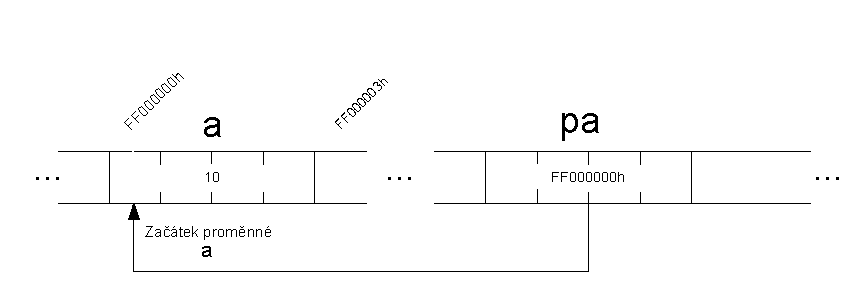
\includegraphics[width=135mm]{princip_ukazatele.pdf}
      \caption{Princip ukazatele v paměti}
      \label{figure:pointer1}
    \end{figure}
    \begin{example}Vytvořte funkce kopírující prvky jednoho pole do druhého pomocí indexu i ukazatele.
    
      \marginpar{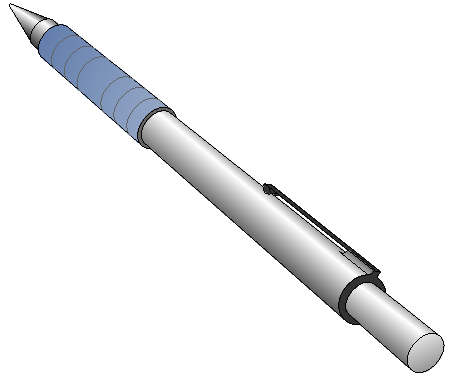
\includegraphics[width=0.09\textwidth]{pen.pdf}}    
      %---------------------------------------------------------------
      \lstinputlisting{../src/C/file/CPYARRY.C}
      \begin{lstlisting}[caption=\texttt{CPYARRY.C} Kopíruje prvky jednoho pole do druhého.]
      \end{lstlisting}
      %---------------------------------------------------------------
      Výstup programu:                                                     \newline
        \lstinline[basicstyle=\ttfamily]!1   2   3   4   5   6   7   8   9!\newline
        \lstinline[basicstyle=\ttfamily]!1   2   3   4   5   6!            \newline
        \lstinline[basicstyle=\ttfamily]!4   5   6   7   8   9!            \newline
    \end{example} 